\chapter{Studie}
\section{Android}
Android ist, im Gegensatz zu anderen mobilen Betriebssystemen auf dem Markt, eine offene Plattform. Das kommt im Wesentlichen daher, dass Android auf einem open source System, dem Linux Kernel, aufbaut. Durch die freie Verfügbarkeit des Codes, gibt es im Android-Bereich eine große Developer Szene die laufend eigens modifizierte Betriebssysteme (ROMs) und Apps hervorbringt.
Ein so hoher Grad an Offenheit birgt jedoch auch gewisse Sicherheitsrisiken und öffnet Angriffsvektoren. Um diese Gefahren besser zu verstehen sollte man sich eingehend mit der Android Architektur und dem darin enthaltenen Sicherheitskonzept befassen.

\subsection{Architektur}
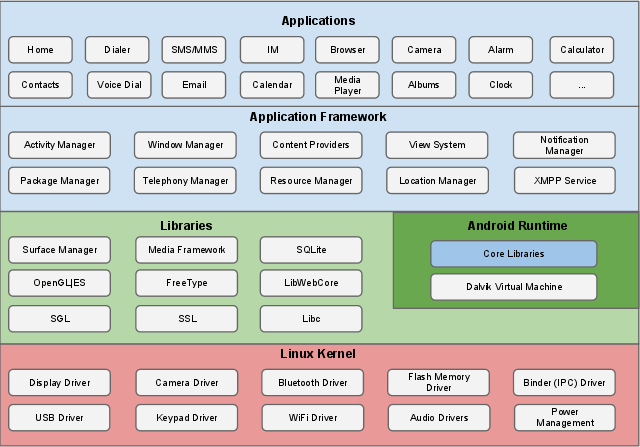
\includegraphics[scale=0.7]{Images/android_stack}
%\caption[Android Architektur Schichtenmodell]{Android Architektur }
\paragraph*{}
Wie in Abbildung 1 zu sehen ist, bildet der Linux Kernel die unterste Schicht der Architektur. Auf ihm baut das gesamte Betriebssystem mitsamt aller Sicherheitskonzepte auf. Der Kernel stellt die Brücke zwischen Hard- und Software dar und enthält die Treiber für diverse andere Komponenten eines Smartphones wie beispielsweise Modem, GPS Empfänger, Kamera, etc… 
\paragraph*{}
In der darüber liegende Ebene sind die Android Libaries sowie die Runtime, also die „Dalvik Virtual Machine“ zu finden. \newline
Android Apps sind meist in Java Programmiert und werden jeweils in einer eigenen Virtuellen Maschine ausgeführt, der DVM \footnote{Dalvik Virtual Machine}. Diese Systematik ermöglicht das logische, parallele, unabhängige Ausführen von verschiedenen Apps mit verschiedenen Benutzerrechten.
Die Libaries steuern und kontrollieren im Wesentlichen die Funktionen des Kernels und sind für die zentralen Funktionalitäten auf niedriger Ebene zuständig.
\paragraph*{}
Die nächst-höhere Ebene bildet das Application Framework. Hier befinden die Grundfunktionen von Android wie zum Beispiel Telefonie, Location Services, Window Manager, Notification Manager, etc… 
Auf dieser Ebene werden Entwicklern äußerst umfangreiche APIs für das Entwickeln von Benutzeranwendungen (Apps) zur Verfügung gestellt.
\paragraph*{}
Die oberste Schicht in der Android-Systemarchitektur sind die Applikationen welche der Benutzer selbst installiert und auf den darunterliegenden Schichten aufbaut.
\paragraph*{}
Dieser gesamte „Stack“ (=Stapel) wird in einem ROM zusammengefasst und auf ein Smartphone installiert. Durch die zuvor erwähnte Offenheit des Systems können so durch Modifizieren eines ROM Paketes stark angepasste Versionen von Android entwickelt und verwendet werden.


\subsection{Security}
Android wird als Betriebssystem mittlerweile auf ca 84\% aller Smartphones weltweit eingesetzt. \footnote{Quelle: http://www.idc.com/prodserv/									smartphone-os-market-share.jsp Stand Q3 2014} Ein Betriebssystem mit einem so großen Marktanteil erfordert ein durchdachtes und ausgereiftes Sicherheitskonzept.
Die drei grundlegenden Sicherheitsobjekte sind:

\begin{itemize}
	\item Schützen von Benutzerdaten
	\item Schützen von Systemressourcen (inklusive Netzwerk)
	\item Bereitstellen von Applikationsisolation
\end{itemize}
Um diese Objekte zu erreichen, stehen eine Reihe von Security-Features zur Verfügung
\begin{itemize}
	\item Robuste Security auf der OS Ebene durch den Linux Kernel
	\item Erforderliche Sandbox für alle Apps
	\item Sichere interprozess Kommunikation
	\item Application signing
	\item Application-defined and user-grated permissons
\end{itemize}

\subsubsection{System- und Kernel Security}
Der Linux Kernel stellt das Fundament von Android dar. Durch dessen langjährige Wartung und Weiterentwicklung hat dieser sich zu einem äußerst sicheren und weit verbreiteten Kernel entwickelt, welcher auch in Sicherheitsempfindlichen Umgebungen eingesetzt wird.
\paragraph*{}
Der Linux Kernel stellt einige der wichtigsten Sicherheitsfunktionen zur Verfügung.
\begin{itemize}
	\item Ein Benutzer-basiertes Rechtemodell
	\item Prozessisolation
	\item Mechanismus für sichere IPC \footnote{Interprozesskommunikation} 
	\item Die Möglichkeit potentiel gefährliche Teile des Kernels zu entfernen
\end{itemize}
Im Gegensatz zum normalen Linux, wo mehrere Anwendungen mit demselben Benutzer ausgeführt werden, weist Android jeder Applikation eine eigene User ID zu und führt diese mit ebendiesem User in einem separaten Prozess aus.
Diese Vorgehensweise resultiert in einer „Kernel-level Application Sandbox“. Dadurch kann eine App von Haus aus mit keiner anderen App kommunizieren sofern dies nicht explizit erwünscht ist. Standardmäßig können Apps auch nicht auf Dinge wie Standort, die Telefonie-Funktion, etc. zugreifen sondern müssen erst um die Erteilung der entsprechenden Benutzerrechte ansuchen. Die Tatsache dass diese Sandbox-Systematik auf Jahrzehnte alter UNIX Technologie aufbaut, macht das System leicht überwachbar und transparent, jedoch gleichzeitig effizient.
\paragraph*{}
Speicherfehler führen in vielen Betriebssystemen zu groben Sicherheitsrisiken und sind in der Lage die Sicherheit eines Gerätes komplett zu kompromittieren. Bei Android kann ein solcher Speicherfehler durch das Sandboxing aller Applikationen auf OS-Level keinen allzu großen Schaden anrichten, da eventueller Schadcode nur im Kontext einer bestimmten App, mit eingeschränkten Benutzerrechten ausgeführt werden kann.
\paragraph*{}
Selbstverständlich ist auch die Applikations-Sandbox nicht zu 100\% sicher, möchte man diese aber knacken, so muss man es schaffen den gesamten Linux Kernel zu kompromittieren.
	
\subsection{Probleme}